\chapter{Results and Analysis}
\label{Chapter:Results}

\section{Serpent Model}
The actuator characterization methodology described in Section \ref{Section:Serpent} is extensive and computationally expensive. Before conducting the main study, some simpler codes were run to ensure that these efforts were spent on a viable design. The reactor must have adequate excess reactivity to overcome equilibrium poisoning and several years of depletion. Conversely, adequate shut-down margin is required to ensure that the reactor can be scrammed even in the event of a partial failure to the control drum drives. Finally, as the \acs{msnb} is meant to operate for extended periods of time without significant maintenance, the control material should still be effective at the end of the reactor lifetime. With the results of these three simple studies in mind, the neutron spectra in key regions of the \acs{msnb} are investigated to recommend improvements to the design that may warrant future work.

\subsection{Excess Reactivity and Shut-down Margin}
Excess reactivity is calculated by orienting the \acs{msnb} in its most reactive control position with fresh fuel and running a criticality model. The neutron multiplication factor (k\textsubscript{eff}) predicted by Serpent is converted to reactivity, and the magnitude above zero is reported as the excess reactivity of the design: 

\begin{equation}
    \rho = \frac{k_{eff}-1}{k_{eff}}
\end{equation}

After several iterations, the design used in this work was found to have an excess reactivity of 4.834\% $\pm$ 45.3 pcm with an average core temperature of 650 \textsuperscript{o}C. This is generally considered to be a slim margin, although the relatively low specific power reduces the equilibrium poison levels and the rate of fissile depletion, and aligns with previous work conducted on a similar design \cite{PetersonMS}. In this work, the initial batch of fuel lasted nearly 6 years before the total loss of excess reactivity was observed.

\begin{figure}[!ht]
    \centering
    \subfloat[\centering Single Misfire]{\includegraphics[width=0.48\textwidth]{Plotter/0.0shutdown7drum/MSNB_geom4}}
    \subfloat[\centering Single Success]{\includegraphics[width=0.48\textwidth]{Plotter/0.0shutdown1drum/MSNB_geom4}}
    \caption[X-Y View of \acs{msnb} - Shut-Down Margin]{X-Y Views of \acs{msnb} with control drums in two shut-down margin failure modes:
    \begin{enumerate*}[label=\alph*)]
        \item Seven drums in least reactive orientation, one drum failed in most reactive orientation; and 
        \item One drum in least reactive orientation, seven drums failed in most reactive orientation; 
    \end{enumerate*}
    The entire wedge of each control drum is colored for clarity. Only the outer rim is actually made from boron carbide.}
    \label{fig:Plotter-SDM}
\end{figure}

The shut-down margin is found using a similar methodology, placing the \acs{msnb} in a very low reactivity orientation and observing the results of the criticality model. With all 8 control drums facing inward, this design has a 54.76\% $\pm$ 103 pcm shut-down margin. This is an extremely high shut-down margin, meaning that only a fraction of the reactor's available control reactivity is needed to carry-out an emergency shut-down. 

\acsp{lwr} are required to maintain 1\% shut-down margin with the most reactive control rod failing to actuate \cite{Margin}. Two further case studies were conducted, as depicted by Figure \ref{fig:Plotter-SDM}, to study the effect of actuation failures. First, a shut-down margin of 47.19\% $\pm$ 91.0 pcm was calculated for the \acs{msnb} in the event that one of the control drums is stuck in its most reactive orientation. Then, a worst case scenario, where only one control drum successfully actuates was found to have a shut-down margin of 0.417\% $\pm$ 46.4 pcm with fresh, un-poisoned fuel. It is extremely unlikely that 7 out of 8 drums would fail to actuate in an emergency, assuming a well designed fail-safe and redundant system. Even in this unlikely event, the \acs{msnb} could be safely shut-down.

\subsection{Control Material Longevity}
Boron carbide was selected as the control material for this design because it simultaneously provided adequate shut-down margin and excess reactivity. It is, however, a burnable neutron poison, meaning that a \B[10] atom can only absorb one neutron. In the interest of keeping maintenance to the \acs{msnb} to a minimum, the control drums cannot lose their ability to insert control reactivity during the expected life of the reactor. The control material was burned at full power (10 MWth) for ten years, and the change to the concentrations of key nuclides were plotted in Figure \ref{fig:BoronBurn}.

\begin{figure}[ht!]
    \centering
    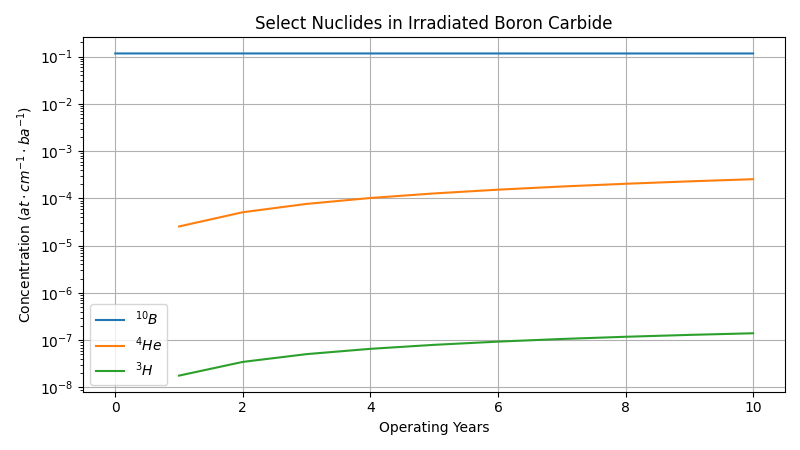
\includegraphics[width=0.9\textwidth]{./Plotter/boronburn/AtomDens}
    \caption[\acs{msnb} Irradiated Boron Carbide]{Concentration of tritium, helium-4, and boron-10 in irradiated boron carbide during a decade-long \acs{msnb} deployment.}
    \label{fig:BoronBurn}
\end{figure}

After 100 MW-yr of heat output, just 0.22\% of the \B[10] was consumed. This caused a negligible effect on the reactivity worth of each control drum. In addition to the deactivation of the neutron poison itself, two gases of interest are formed in boron carbide under neutron fluence. Helium-4 is formed after the alpha particle from the primary capture reaction is de-ionized:

\begin{reaction} \label{rxn:B10cap}
    ^{10}B + n \to {^{7}Li} + \alpha
\end{reaction}

By the end of the decade scale operation, 58 moles of helium have been formed by this pathway. This is a significant amount that will need to be off-gassed operation, and could cause swelling if the material is not properly qualified. Tritium is also formed both directly and indirectly by the $^{10}B(n,2\alpha){^{3}H}$ and $^{7}Li(n,n\alpha){^{3}H}$ reactions. At the end of the study, the control material of the \acs{msnb} contained 31.9 millimoles, or 95.7 mg of tritium. This will account for a small amount of the total radioactivity in the decommissioned \acs{msnb}.

\subsection{Neutron Spectra}
A detector code was used to study the volume average neutron flux in three concentric regions. A material detector card was specified for:
\begin{enumerate*}
    \item the molten salt in the core;
    \item the reflector; and
    \item the molten salt in the downcomer.
\end{enumerate*}
500 energy bins of equal lethargy\footnote{Neutron lethargy is a logarithmic energy ratio. Energy bins of equal lethargy width are uniformly distributed when plotted on a log-axis.} width from 10 $\mu$eV to 20 MeV. Figure \ref{fig:Spectrum} displays the neutron spectra in the three regions within the \acs{msnb}.

\begin{figure}[ht!]
    \centering
    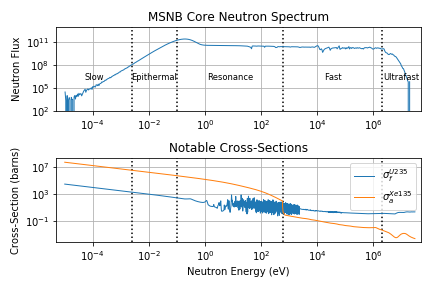
\includegraphics[width=0.9\textwidth]{./Plotter/Detector/Spectrum}
    \caption[\acs{msnb} Neutron Energy Spectrum]{\raggedright \acs{msnb} neutron energy spectrum in core, reflector, and downcomer.}
    \label{fig:Spectrum}
\end{figure}

The \acs{msnb} is a fast/epithermal reactor. Most fission neutrons that are emitted at ~2 MeV are not fully thermalized, as they are in \acsp{lwr}. Within the core, The volume average flux generally diminishes as the neutron energy drops, with some discontinuities caused by major resonance peaks of \F, \Li[7], \Na, \K, \U[235], and \U[238], the major constituents of the molten salt fuel. For most neutron energies, the volume average flux in the downcomer is about 2 orders of magnitude, indicating leakage of approximately 1\%. 

An epithermal peak of about 0.1 eV is observed in the downcomer and reflector. The corresponding peak is much smaller in the core spectrum. This implies that this design is not optimally moderating neutrons in the core, \ie the lower energy neutrons have small path length inside the core. This is likely because those neutrons that transport to the edge of the core, are slowed in the reflector, and re-enter the core do not penetrate deep into the core before inducing fission or being captured. Because the \acs{msnb} has ample shut-down margin and limited excess reactivity, it is recommended that in future work, a wider diameter core with smaller flow paths surrounded by in-pile moderation is designed. This will allow the core to make better use of the epithermal peak that is caused by the beryllium oxide reflector, increase the overall macroscopic fission cross-section, and produce a more reactive core.


\subsection{Actuator Curve}\label{sec:actuator}

\begin{figure}[!ht]
    \centering
    \subfloat[\centering Xenon-135 Build-up]{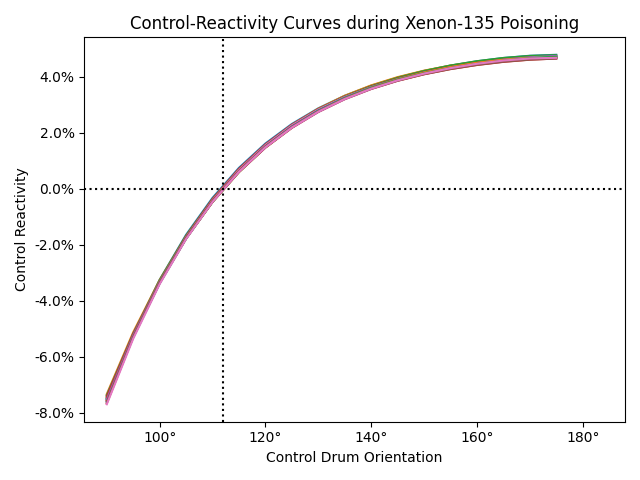
\includegraphics[width=0.49\textwidth]{/CurveFits/eqXe}}
    \subfloat[\centering Depletion]{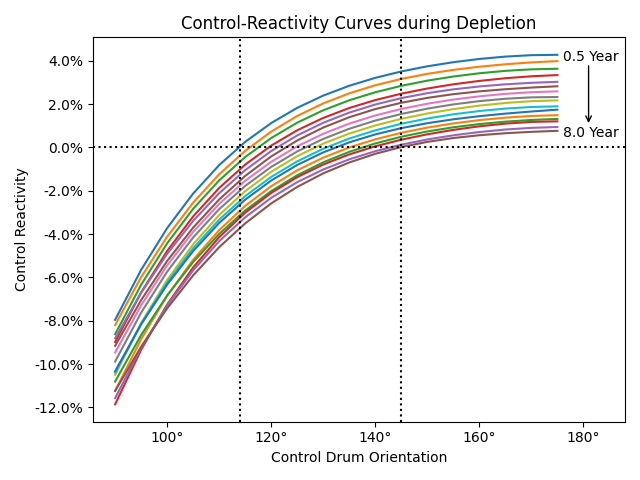
\includegraphics[width=0.49\textwidth]{/CurveFits/depletion}}
    \caption[Control Reactivity Curve]{Control drum angle vs. reactivity curves. Each curve corresponds to a different burn-up level:
    \begin{enumerate*}[label=\alph*)]
        \item 6 hour increments until \Xe reaches equilibrium`'; and 
        \item 6 month increments until the fuel is depleted enough that the \acs{msnb} has very little excess reactivity; 
    \end{enumerate*}
    }
    \label{fig:ControlReactivityCurve}
\end{figure}

The controller that is tuned and studied in Section \ref{sec:simulation} depends on a detailed actuator characterization. The \acs{msnb}'s static response to the orientation of the control drums were studied over the life of the reactor in an alternating methodology of criticality and burn-up modeling, detailed in Section \ref{Section:Serpent}. Figure \ref{fig:ControlReactivityCurve} depicts the evolution of the core reactivity vs. the rotational angle of the control drum as the \Xe level rises to equilibrium, and as the \U[235] is depleted. The controller model treats the control drum as an \acs{lti} system. The figure clearly shows that the actuator response is neither linear nor time-invariant. Over time, the reactor's response to the actuator changes, however, these are not rapid changes; the \Xe worth at equilibrium for the specific power of study (10 MW) is small enough that the curves overlap, with only dozens of pcm separating the fresh and poisoned fuel. Furthermore it takes eight years for the unity point to drift by approximately 20 degrees. The evolution of the actuator response can easily be modeled using a look-up table. The controller will set a different bias and use a different gain depending on the length of time that the \acs{msnb} has operated. The data was fit to a series of fourth order polynomials which the process simulator can use to calculate the control reactivity ($\rho$) given the control drum orientation ($\theta$):

\begin{equation}
    \rho = c_0 + c_1\theta + c_2\theta^2 + c_3\theta^3 + c_4\theta^4
\end{equation}

During normal operation, the reactor will only be made slightly supercritical to power up or subcritical to power down, likely on the order of tens to hundreds of pcm. This corresponds to a small rotation of the control drums. For the purposes of controller design, the control-reactivity curve can be linearized simply by solving for the root of the polynomial and computing the derivative at that point. The root of the curve corresponding to the current depth of burn-up will be set as the controller bias, while the slope of the tangent line (in pcm/degree) can be used to scale the controller gain (in degree/kW) and obtain the desired combined controller-actuator gain (in pcm/kW). Notably, the root of all of the curves lies above its inflection point. As a result the actuator will insert less positive reactivity than the controller intends during an up-transient, land more negative reactivity than the controller intends during a down-transient. The deviation between the polynomial and linearization is small for the expected range of control drum orientations, but this may result in slightly better performance when increasing the power duty. The polynomial coefficients defining the curves and root/tangent slope are listed in Tables \ref{tab:Xefit} and \ref{tab:Depletionfit}. $c_0$ could be adjusted to account for a different operating temperature, which would shift the curve up or down according to $\alpha_t$, and require re-linearization around the new root. 

\begin{table}[t!]
    \caption[Control Reactivity Curve Fit - Equilibrium Poisoning]{Polynomial coefficients, root, and slope for the control drum vs. reactivity curves during equilibrium poisoning.}
    \centering\begin{tabular}{c|ccccc|cc}
    \hline
    Hours & c\textsubscript{4} \sci[9] & c\textsubscript{3} \sci[6] & c\textsubscript{2} \sci[4] & c\textsubscript{1} \sci[2] & c\textsubscript{0} & root ($^o$) & slope ($pcm/^o$) \\ \hline
    0  & -2.797 & 1.789 & -4.361 & 4.829 & -2.009 & 111.41 & 224.24 \\
    6  & -2.076 & 1.372 & -3.475 & 4.005 & -1.727 & 111.71 & 221.35 \\
    12 & -2.701 & 1.725 & -4.211 & 4.676 & -1.953 & 111.61 & 221.89 \\
    18 & -2.780 & 1.797 & -4.393 & 4.874 & -2.031 & 111.63 & 224.23 \\
    24 & -2.292 & 1.501 & -3.753 & 4.265 & -1.817 & 111.97 & 218.62 \\\hline
    30 & -2.226 & 1.470 & -3.706 & 4.244 & -1.819 & 111.94 & 222.27 \\
    36 & -2.116 & 1.424 & -3.643 & 4.211 & -1.814 & 111.77 & 223.04 \\
    42 & -2.086 & 1.376 & -3.483 & 4.009 & -1.728 & 112.02 & 217.91 \\
    48 & -2.330 & 1.517 & -3.776 & 4.277 & -1.819 & 112.09 & 217.58 \\\hline
    54 & -2.174 & 1.439 & -3.635 & 4.168 & -1.788 & 112.04 & 219.12 \\
    60 & -2.287 & 1.508 & -3.797 & 4.334 & -1.851 & 111.96 & 221.58 \\
    66 & -2.696 & 1.716 & -4.178 & 4.636 & -1.937 & 112.00 & 218.60 \\
    72 & -1.990 & 1.332 & -3.406 & 3.951 & -1.712 & 112.08 & 217.56 \\\hline
    78 & -2.227 & 1.464 & -3.674 & 4.190 & -1.791 & 112.07 & 216.57 \\
    84 & -2.665 & 1.704 & -4.162 & 4.626 & -1.935 & 111.98 & 217.40 \\
    90 & -2.627 & 1.696 & -4.177 & 4.668 & -1.958 & 111.88 & 220.09 \\
    96 & -2.859 & 1.818 & -4.413 & 4.870 & -2.023 & 112.05 & 219.42 \\
    \end{tabular}
    \label{tab:Xefit}
\end{table}

\begin{table}[bh!]
    \caption[Control Reactivity Curve Fit - Fuel Depletion]{Polynomial coefficients, root, and slope for the control drum vs. reactivity curves during fuel depletion.}
    \centering\begin{tabular}{c|ccccc|cc}
    \hline
    Years & c\textsubscript{4} \sci[9] & c\textsubscript{3} \sci[6] & c\textsubscript{2} \sci[4] & c\textsubscript{1} \sci[2] & c\textsubscript{0} & root ($^o$) & slope ($pcm/^o$) \\ \hline
    0.0 & -2.797 & 1.789 & -4.361 & 4.829 & -2.009 & 111.41 & 224.24 \\
    0.5 & -2.755 & 1.755 & -4.272 & 4.732 & -1.976 & 113.69 & 203.69 \\
    1.0 & -1.838 & 1.253 & -3.253 & 3.826 & -1.682 & 115.79 & 189.71 \\
    1.5 & -2.533 & 1.632 & -3.253 & 4.507 & -1.909 & 117.38 & 175.96 \\
    2.0 & -2.418 & 1.578 & -3.930 & 4.440 & -1.895 & 119.45 & 161.06 \\\hline
    2.5 & -1.461 & 1.026 & -2.750 & 3.337 & -1.515 & 121.06 & 152.71 \\
    3.0 & -1.137 & 0.856 & -2.425 & 3.070 & -1.440 & 122.67 & 146.08 \\
    3.5 & -2.054 & 1.357 & -3.433 & 3.953 & -1.727 & 124.58 & 130.85 \\
    4.0 & -2.527 & 1.617 & -3.967 & 4.438 & -1.892 & 126.46 & 120.67 \\\hline
    4.5 & -2.869 & 1.831 & -4.460 & 4.935 & -2.081 & 128.35 & 111.30 \\
    5.0 & -2.338 & 1.520 & -3.785 & 4.291 & -1.855 & 130.55 & 102.04 \\
    5.5 & -1.471 & 1.054 & -2.852 & 3.467 & -1.585 & 132.29 & 93.34 \\
    6.0 & -2.626 & 1.702 & -4.211 & 4.729 & -2.027 & 134.96 & 83.90 \\\hline
    6.5 & -1.672 & 1.141 & -2.985 & 3.550 & -1.607 & 137.45 & 77.56 \\
    7.0 & -3.321 & 2.095 & -5.036 & 5.492 & -2.292 & 139.19 & 69.73 \\
    7.5 & -2.419 & 1.579 & -3.936 & 4.459 & -1.932 & 142.69 & 59.45 \\
    8.0 & -7.991 & 0.648 & -1.960 & 2.623 & -1.305 & 144.62 & 55.65 \\
    \end{tabular}
    \label{tab:Depletionfit}
\end{table}

\section{Multi-physics Simulation}\label{sec:simulation}
A series of case studies were conducted on the \acs{msnb} using the multi-physics process simulation. For each case study, the autonomous response was observed to use as a base case against the controlled response. In the autonomous response, the core to responds to heat exchanger transients only by passive (temperature and flow reactivity) feedback mechanisms, as the controller is turned off. In the controlled response, the control drums insert active feedback in response to error. The passive feedback mechanisms alone are then compared with the addition of the \acs{pid} controller quantitatively by analyzing the relative magnitude of the inverse response and first two overshoot peaks, as well as the delay time, rise time, settling time, and oscillation period. 

The delay time and rise time are the times it takes for the core power to change by 10\% and 90\% of the heat exchanger step size, respectively. The settling time is the time it takes for the core power oscillations to converge to a bandwidth of $\pm$5\% of the heat exchanger step size centered on the new set-point. The oscillation period is recorded as the time between the first and second overshoot peak. These metrics capture the shape of the response curve, and allow for quantitative comparisons of a rather intuitive nature; to facilitate high-fidelity load-following in the operation of the \acs{msnb}, a short delay time, rise time, and settling time, as well as a small inverse response and small overshoot. 

In addition to the trivial steady-state base case, five transients are studied:
\begin{enumerate*}
    \item A step from 8 MW to 10 MW;
    \item A step from 10 MW to 8 MW;
    \item A start-up, where the \acs{msnb} is ramped from hot-standby (100 kW) to low-power (1 MW), then from low-power to full-power (10 MW);
    \item A shut-down, where the \acs{msnb} is ramped from full-power to low-power, then to hot-standby;
    \item A demand response, where the \acs{msnb} is ramped from 8 MW to 10 MW, then back to 8 MW;
\end{enumerate*}

Each of these transients is studied below, and key figures are presented for discussion. The process simulator plots many data sets each time it is run. Each of these plots are available for further observation on GitHub\footnote[2]{All figures generated for each case study are available at https://github.com/sjroot97/MsNB-Simulator/tree/main/CaseStudies}


\subsection{Steady-State}
\begin{figure}[ht!]
    \centering
    \includegraphics[width=0.9\textwidth]{Simulator/SteadyState/t_vs_Qt}
    \caption[Steady state power response]{Core power response to a steady heat exchanger demand of 10 MW given the initial conditions.}
    \label{fig:SS-Power}
\end{figure}

Before studying transients, steady-state operation was tested. The \acs{msnb} was held constant at 10 MW for a full hour. The slight error between the initial temperature profile guess and the temperature profile to which simulation converges kicks off core power oscillation, as shown by Figure \ref{fig:SS-Power}. The first peak results in a momentary offset of nearly 200 kW (0.2\% nominal error), and roughly one-third wave decay is observed with a period of approximately 6 minutes. The offset is essentially `rung-out' within 40 minutes.

Figure \ref{fig:SS-Velocity} shows that the initial velocity guess is about 0.8 mm/s slower than the convergent velocity. This is caused by minor disturbances to the temperature profile. The assumption of uniform temperature rise in the core and uniform temperature decrease in the heat exchanger is not completely accurate due to the temperature functions of specific heat and density. A more accurate initial guess may to assume uniform change to the internal energy of each control volume, however the stability of the curves implies that the assumption is adequate. Approaching steady-state core output, the velocity profile has quite a high frequency; this is likely due to the way that the velocity is calculated. Buoyant forces are negated by frictional losses for each time-step. This is a first-order approach. A second-order approach would consider the net force resultant from changing buoyancy and accelerate the fluid according to Newton's second law. The fluid inertia would increase the oscillatory period and likely dampen the response. The sustained oscillation of the power profile, as well as the `kick' at 56 minutes are likely a result of the `advection only' approach to heat convection employed by the simulator. Thermal diffusion would smooth out the temperature profile and eliminate the anomalies that delay the simulated \acs{msnb} from fully reaching steady-state operation.

\begin{figure}[ht!]
    \centering
    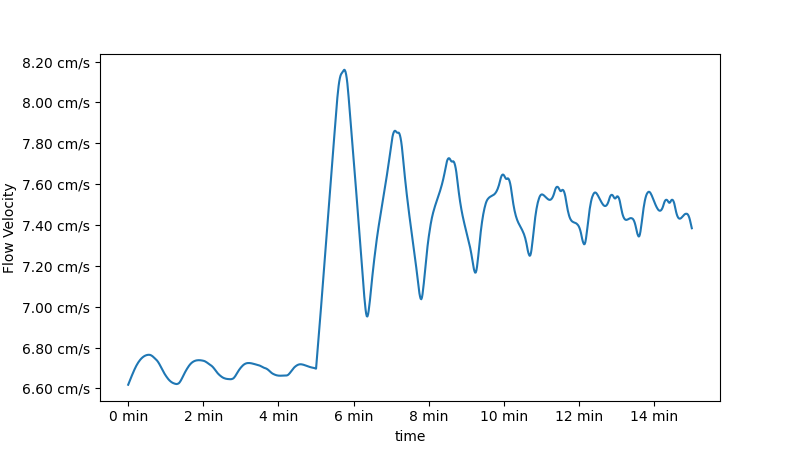
\includegraphics[width=0.9\textwidth]{Simulator/SteadyState/t_vs_velocity}
    \caption[Steady state velocity response]{Core velocity response to a steady heat exchanger demand of 10 MW given the initial conditions.}
    \label{fig:SS-Velocity}
\end{figure}

Even with these limiting assumptions, the trivial case study provides confidence that the multi-physics model adequately describes the stable passive feedback mechanisms that couples the nuclear kinetics of the \acs{msnb} to its thermal hydraulic phenomena. The simulation is self-stabilizing against small excursions, and can reasonably be expected to respond to larger transient studies so long as the magnitude is not de-stabilizing.

\subsection{Up-Step}
The first transient of study is a simple step from 8 MW to 10 MW. This is an instantaneous change of 25\%, and is likely much more aggressive than will ever actually be required in practice. Step functions are, however, useful for controller tuning and performance assessment, making this a valuable study even if it is more likely for this system to respond to ramp functions.

\subsubsection{Autonomous Response}
Figure \ref{fig:Up-Power-Auto} displays the core response to the heat exchanger up-step that results from only passive feedback. The defining feature of this plot is the inverse response immediately after the heat exchanger step that is caused by the increased natural circulation flow rate as the cold leg cools. Faster flow causes a negative flow reactivity insertion and makes the \acs{msnb} subcritical until the cold salt reaches the core and temperature reactivity ramps up the core power. 

These dynamics are readily apparent on Figure \ref{fig:Up-Reac-Auto}, where the initial dip in total reactivity appears only on the flow reactivity line. As the core power increases, hotter and hotter salt propagates around the flow loop, eventually raising the average core temperature enough that the reactor goes subcritical, and the core power rounds the first overshoot peak. 

\begin{figure}[ht!]
    \centering
    \includegraphics[width=0.9\textwidth]{Simulator/StepUp/Auto/t_vs_Qt}
    \caption[Autonomous Up-Step Power Response]{\raggedright Autonomous core power response to a heat exchanger demand step function from 8 MW to 10 MW.}
    \label{fig:Up-Power-Auto}
\end{figure}

When the core power dips below the heat exchanger power, salt cooling, governed by the transport delay problem, begins to ramp the core power back up, and the dynamics repeat, with smaller and smaller overshoot peaks each cycle. The key metrics obtained from analyzing Figure \ref{fig:Up-Power-Auto} are:

\begin{itemize}
    \item Delay Time - 1.2 min;
    \item Rise Time - 2.3 min;
    \item Settling Time - 40.5 min;
    \item Oscillation Period - 6.5 min;
    \item Inverse Response - 27.5\%;
    \item First Overshoot - 105.0\%;
    \item Second Overshoot - 57.5\%;
\end{itemize}

The large overshoots, roughly half-wave decay, and long settling time are indicative of a rather poor autonomous response to this transient. Notably, the reactor handles this poor response without being destabilized, causing reverse flow, or approaching thermophysical limits of the molten salt. 

\begin{figure}[ht!]
    \centering
    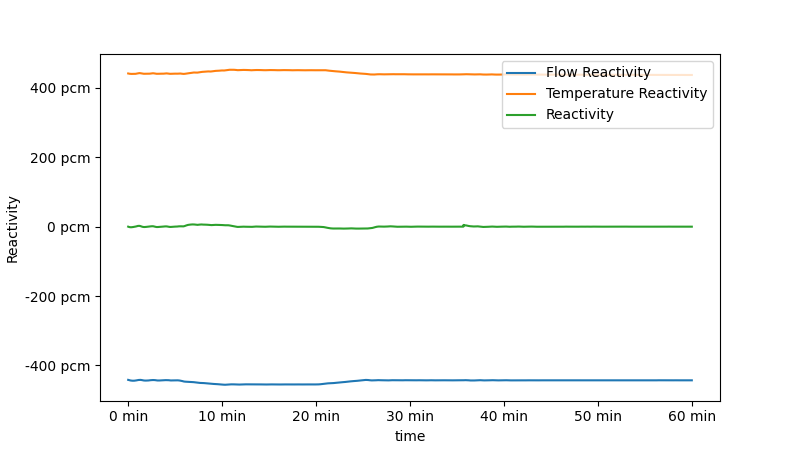
\includegraphics[width=0.9\textwidth]{Simulator/StepUp/Auto/t_vs_reac}
    \caption[Autonomous Up-Step Reactivity Response]{Autonomous core reactivity response to a heat exchanger demand heat exchanger demand step function from 8 MW to 10 MW.}
    \label{fig:Up-Reac-Auto}
\end{figure}

\subsubsection{Controller Tuning}
The controller was tuned using the Ziegler-Nichols methodology. This common closed loop tuning methodology requires placing the controller in P-only mode and increasing the proportional gain ($K_p$) until the response exhibits sustained oscillations. The gain at which this occurs is defined as the ultimate gain, and the period of oscillation is the ultimate period. Recommended \acs{pid} gains and time constants can be obtained from these values. The desired behavior was approached with a $K_p$ of 3 $\times$ 10\textsuperscript{-4} degree/kW and the fresh fuel control-reactivity curve, and resulted in an ultimate period of 45 seconds. 

Several of the recommended \acs{pid} gains were tested, and it was observed that all with a significant derivative time constant destabilized the \acs{msnb}. Therefore, it was decided to use the \acs{pi} controller recommendations, effectively setting the derivative time constant to zero. A $K_p$ of 1.35 $\times$ 10\textsuperscript{-4} degree/kW (which corresponds to a combined controller-actuator gain 30.3 pcm/MW) and $\tau_I$ of 37.5 seconds provided a stable response to all of the transients of study with acceptable performance. It is likely that finer tuning of these parameters could slightly improve the performance of the controller, however a more refined loop shaping analysis focused on the poles and zeros of the overall loop transfer function would be a better approach likely to yield superior results. A publication investigating an advanced controller design of this nature will follow this thesis.

\subsubsection{Controller Response}
The case study was repeated with the Ziegler-Nichols tuned \acs{pi} controller. In observing Figure \ref{fig:Up-Power-Ctr}, it is apparent that the inverse response is completely eliminated and the peak overshoot is significantly reduced. The simulation length has been reduced to display greater detail of the response, as the settling time and oscillation period are both greatly reduced:

\begin{itemize}
    \item Delay Time - 0.6 min;
    \item Rise Time - 1.1 min;
    \item Settling Time - 5.3 min;
    \item Oscillation Period - 1 min;
    \item Inverse Response - 0.0\%;
    \item First Overshoot - 11.5\%;
    \item Second Overshoot - 14.5\%;
\end{itemize}

\begin{figure}[ht!]
    \centering
    \includegraphics[width=0.9\textwidth]{Simulator/StepUp/Control/t_vs_Qt}
    \caption[Controlled Up-Step Power Response ]{\raggedright Controlled core power response to a heat exchanger demand step function from 8 MW to 10 MW.}
    \label{fig:Up-Power-Ctr}
\end{figure}

This represents nearly a 100\% improvement to the delay and rise time (which is limited by the pre-filter) and an order of magnitude improvement to the settling time and first overshoot. The second overshoot is greater than the first, but is still significantly smaller than the second peak of the autonomous response, and minor oscillations follow. These oscillations are a result of over-actuation. After the core power settles around the set-point, the control drums are slightly rotated back and forth by 1.5 arc-minutes with a period of about 1 minute. This behavior, displayed by Figure \ref{fig:Up-Drum-Ctr}, is unnecessary and can lead lead to premature wear to the control drum drive motors. In the future, the error and actuator signals could be processed in an effort to stabilize the controller output.

\begin{figure}[ht!]
    \centering
    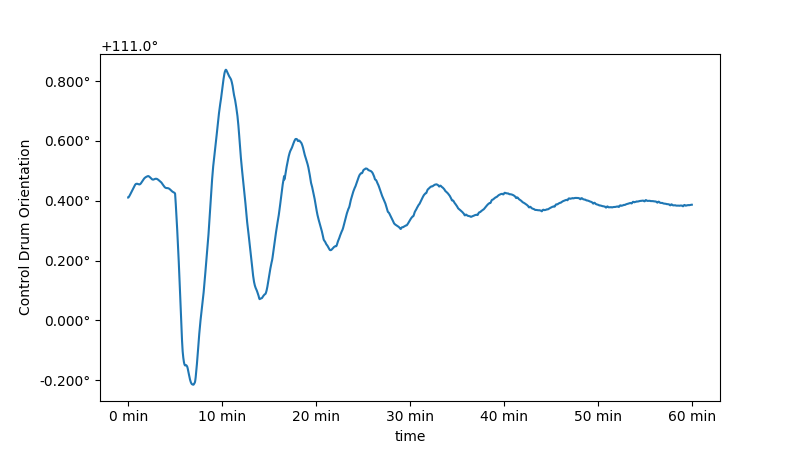
\includegraphics[width=0.9\textwidth]{Simulator/StepUp/Control/t_vs_angle}
    \caption[Up-Step Actuator Response]{\raggedright Control drum angle response to a heat exchanger demand step function from 8 MW to 10 MW.}
    \label{fig:Up-Drum-Ctr}
\end{figure}

\subsection{Down-Step}
To further study the controller, the opposite step function was also studied. Very similar dynamics are expected for a step from 10 MW to 8 MW.

\subsubsection{Autonomous Response}
Figure \ref{fig:Down-Power-Auto} looks very similar to the mirror image of Figure \ref{fig:Up-Power-Auto}, but the inverse response is appreciably larger. This is an artifact of the exponential formula used to calculate flow reactivity. When the heat exchanger power is reduced, the cold leg begins to warm up and the natural circulation flow rate reduces. A reduction in velocity changes the flow reactivity more than an equivalent velocity increase for a given starting velocity. Following the inverse response, the down-step response behaves very similarly to the up-step:

\begin{itemize}
    \item Delay Time - 1.1 min;
    \item Rise Time - 2.2 min;
    \item Settling Time - 38 min;
    \item Oscillation Period - 7.5 min;
    \item Inverse Response - 45.0\%;
    \item First Overshoot - 90.0\%;
    \item Second Overshoot - 50.0\%;
\end{itemize}

\begin{figure}[ht!]
    \centering
    \includegraphics[width=0.9\textwidth]{Simulator/StepDown/Auto/t_vs_Qt}
    \caption[Autonomous Down-Step Power Response]{\raggedright Autonomous core power response to a heat exchanger demand step function from 10 MW to 8 MW.}
    \label{fig:Down-Power-Auto}
\end{figure}

A convenient way to represent the passive reactivity feedback is by leveraging phase-space. Figure \ref{fig:Down-PassivePhase-Auto} plots the temperature reactivity on the x-axis and the flow reactivity on the y-axis. Along the diagonal, the reactor is critical, and the distance from the diagonal that the time-parametric curve is proportional to the degree of sub/supercriticality. 

\begin{figure}[ht!]
    \centering
    \includegraphics[width=0.9\textwidth]{Simulator/StepDown/Auto/auto_reac_phase}
    \caption[Autonomous Down-Step Reactivity Phase Space]{Passive reactivity phase space response to a heat exchanger demand heat exchanger demand step function from 10 MW to 8 MW.}
    \label{fig:Down-PassivePhase-Auto}
\end{figure}

From\note{I'll fix the annotations on the above figure} the starting point, the \acs{msnb} quivers around unity until the step function occurs, when positive flow reactivity is inserted. The phase space shows how this response leads to salt warming and negative temperature reactivity which brings the reactor back to unity. The flow rate quickly equilibrates around the new velocity, after which the average core temperature is the dominant passive feedback mechanism that delays steady state operation.

\subsubsection{Controller Response}
Again, inspection of Figure \ref{fig:Down-Power-Ctr} tells us that the controller eliminates the inverse response and reduces the overshoot and required timescale:

\begin{itemize}
    \item Delay Time - 0.3 min;
    \item Rise Time - 1.2 min;
    \item Settling Time - 5.2 min;
    \item Oscillation Period - 1 min;
    \item Inverse Response - 0.0\%;
    \item First Overshoot - 8.5\%;
    \item Second Overshoot - 17.5\%;
\end{itemize}

\begin{figure}[ht!]
    \centering
    \includegraphics[width=0.9\textwidth]{Simulator/StepDown/Control/t_vs_Qt}
    \caption[Controlled Down-Step Power Response ]{\raggedright Controlled core power response to a heat exchanger demand step function from 10 MW to 8 MW.}
    \label{fig:Down-Power-Ctr}
\end{figure}

In this case study, the second overshoot is more than double the magnitude of the first. This is due to a variety of factors, which can be understood with the help of Figure \ref{fig:Down-ControlPhase-Ctr}. This figure is similar to Figure \ref{fig:Down-PassivePhase-Auto}. The total passive reactivity is combined onto the x-axis, and the active reactivity is placed on the y-axis. Again, a curve below the diagonal corresponds to subcritical operation. When the heat exchanger is stepped, the pre-filter begins moving the core power set-point, and the \acs{pi} controller immediately responds to the error, making the reactor subcritical. As the cumulative and instantaneous error continue to grow, the passive feedback mechanisms (primary flow reactivity) first resist the controller. When the core power crosses over the set-point, the control drums reverse their direction of rotation as the core accumulates sensible heat. 

This sequence draws a large loop in Figure \ref{fig:Down-ControlPhase-Ctr} and a steep line in Figure \ref{fig:Down-Power-Ctr} at about 6 minutes. Eventually,  first overshoot peak cools and slows the salt enough to momentarily bring the \acs{msnb} back above unity. As the instantaneous error shrinks, the controller backs off just as the salt is heated and accelerated enough to drop the core power one more time. The controlled feedback phase space line then finally follows a swirling path towards unity as the core power oscillations ring out. 



\begin{figure}[ht!]
    \centering
    \includegraphics[width=0.9\textwidth]{Simulator/StepDown/Control/contr_reac_phase}
    \caption[Controlled Down-Step Reactivity Phase Space]{Controlled reactivity phase space response to a heat exchanger demand heat exchanger demand step function from 10 MW to 8 MW.}
    \label{fig:Down-ControlPhase-Ctr}
\end{figure}



\subsection{Start-Up}
Next, the \acs{msnb} was analyzed during a start-up from hot-standby to full-power. The reactor is ramped from 100 kW to 1 MW over three hours, held at low-power for an hour, then ramped to 10 MW in one hour.

\subsubsection{Autonomous Response}
Figure \ref{fig:Start-Power-Auto} displays the passive feedback response to start-up. The first ramp is conducted at just 5 kW/min. This is a very conservative transient, but it is necessary because of the large and persistent inverse response. The initial salt velocity is very low, so the acceleration that occurs when the heat exchanger starts cooling down the cold leg inserts a large amount of negative flow reactivity. The reactor power drops nearly to zero, and it takes a long time for the core to cool enough for temperature feedback to ramp power back up. Once this occurs, the \acs{msnb} responds quite well to the first ramp. The rise time is met nearly as soon as the heat exchanger power ramp reaches 90\% of the total, and the core power response settles after just two overshoot peaks:

\begin{itemize}
    \item Delay Time - 63 min;
    \item Rise Time - 141 min;
    \item Settling Time - 218 min;
    \item Oscillation Period - 21 min;
    \item Inverse Response - 11.1\%;
    \item First Overshoot - 7.8\%;
    \item Second Overshoot - 4.4\%;
\end{itemize}

In Figure \ref{fig:Start-Temp-Auto} (a) and (b), it can be observed how the temperature profile stretches and cools as more heat is transported around the flow loop. An animation showing the evolution of the temperature profile with one minute intervals is available in the supplementary materials\footnotemark[2]. At hot-standby, very little power is transported by the molten salt, so the temperature profile is very flat. A temperature differential of about 25 \textsuperscript{o}C is required to drive the required natural circulation flow rate for the \acs{msnb} to equilibrate at low-power.  

\begin{figure}[ht!]
    \centering
    \includegraphics[width=0.9\textwidth]{Simulator/StartUp/Auto/t_vs_Qt}
    \caption[Autonomous Start-Up Power Response]{Core power response for an autonomous start-up from hot-standby. The heat exchanger power is ramped from 100 kW to 1 MW over three hours, then to 10 MW in a subsequent hour.}
    \label{fig:Start-Power-Auto}
\end{figure}

The second ramp is more aggressive with a ramp rate of 150 kW/min, and brings the \acs{msnb} from 10\% power to total power. The core power responds much more quickly, but is not nearly as high-quality for this transient:

\begin{itemize}
    \item Delay Time - 12 min;
    \item Rise Time - 52 min;
    \item Settling Time - 274 min;
    \item Oscillation Period - 11 min;
    \item Inverse Response - 4.4\%;
    \item First Overshoot - 15.0\%;
    \item Second Overshoot - 14.4\%;
\end{itemize}

It takes more than 3.5 hours after the heat exchanger transient concludes for the core to settle, and overshoots more than 15 times before this occurs. Much of the response is truncated on Figure \ref{fig:Start-Power-Auto} to preserve details. Figure \ref{fig:Start-Temp-Auto} (c) clearly shows why it takes so long for the \acs{msnb} to stabilize. Despite roughly reaching the final temperature differential (which defines the natural circulation flow rate), there is a large temperature rise across the downcomer. As the salt flows, the resultant density wave oscillations propagate around the flow loop, periodically upsetting the core through temperature reactivity insertion and withdrawal. Without significant counteraction from flow reactivity in this time period, the decay ratio is very low.

\begin{figure}[!ht]
    \centering
     \subfloat[\centering Hot-Standby]{\includegraphics[width=0.49\textwidth]{Simulator/StartUp/Auto/animateTx_t/t-1}}
    \subfloat[\centering Low Power]{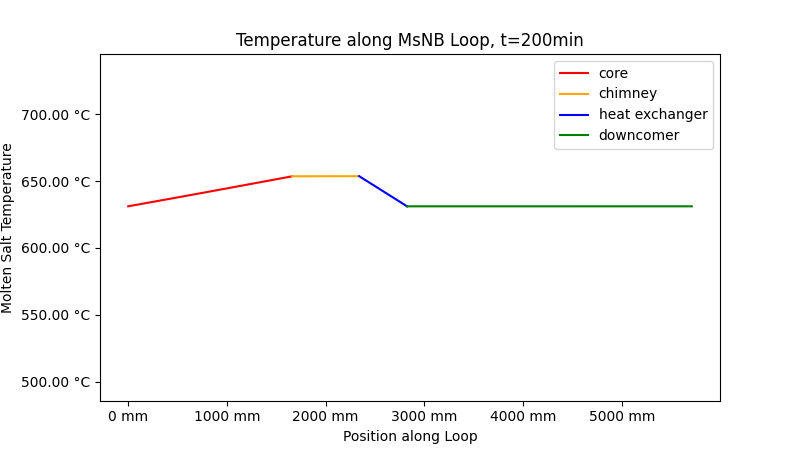
\includegraphics[width=0.49\textwidth]{Simulator/StartUp/Auto/animateTx_t/t-200}}
    \quad
    \subfloat[\centering Full-Power]{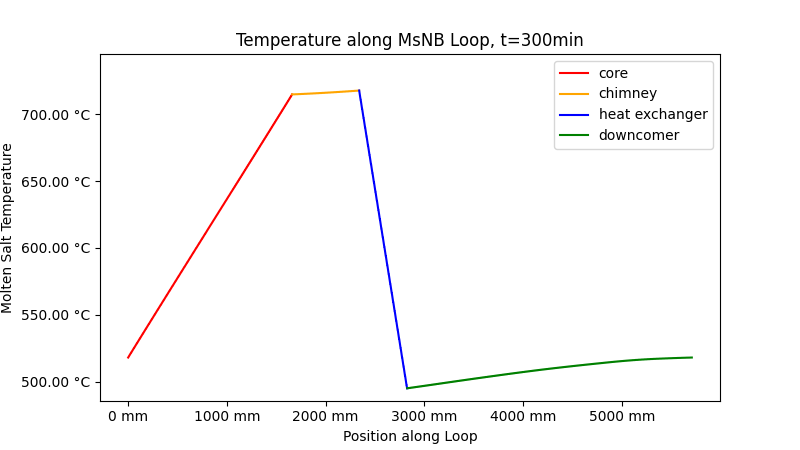
\includegraphics[width=0.49\textwidth]{Simulator/StartUp/Auto/animateTx_t/t-300}}
    \subfloat[\centering Steady State]{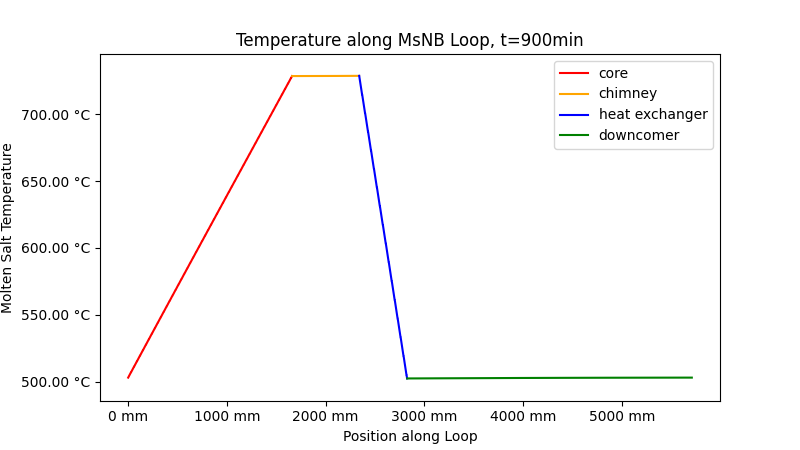
\includegraphics[width=0.49\textwidth]{Simulator/StartUp/Auto/animateTx_t/t-900}}
    \caption[Autonomous Start-Up Temperature Profile Response]{Temperature profile response to an autonomous start-up from hot-standby.
    \begin{enumerate*}[label=\alph*)]
        \item \acs{msnb} is at hot-standby;
        \item \acs{msnb} has equilibrated at 1 MW;
        \item \acs{msnb} has just reached 10 MW; 
        \item \acs{msnb} has equilibrated at 10 MW;
    \end{enumerate*}}
    \label{fig:Start-Temp-Auto}
\end{figure}

Another concerning feature of Figure \ref{fig:Start-Temp-Auto} is the large temperature differential at full-power. The core outlet is over 200 \textsuperscript{o}C hotter than the inlet, which is within 50 \textsuperscript{o}C of the melting point of \flinak, putting the \acs{msnb} at serious risk of \UF recrystallization. The core response needs to be managed to bring the \acs{msnb} to a flow rate and temperature profile more similar to those observed when the simulator starts near full-power.    

\subsubsection{Controller Response}
Even with the benefit of the controller, a large and prolonged inverse response is apparent on Figure \ref{fig:Start-Power-Ctr}. The large and rapid negative flow reactivity is more than the instantaneous controller can effectively counteract. The error remains relatively small because the set-point is so close to zero, and negative power cannot be obtained from a fission source. The controller effectively waits for the cumulative error to build-up before the control drums can overtake the flow reactivity. At this point, the control drums have rotated by more than 1 degree and the actuator linearization begins to over-estimate the expected control reactivity insertion. Despite this issue, the controller is able to shorten the start-up process from 5 hours to 1.5 hours, minimize overshoot and settle the core almost immediately after the set-point converges to the heat exchanger demand. The key metrics for the first ramp are:

\begin{itemize}
    \item Delay Time - 17 min;
    \item Rise Time - 19.5 min;
    \item Settling Time - 40 min;
    \item Oscillation Period - 12 min;
    \item Inverse Response - 11.1\%;
    \item First Overshoot - 27.8\%;
    \item Second Overshoot - 0.5\%;
\end{itemize}

\begin{figure}[ht!]
    \centering
    \includegraphics[width=0.9\textwidth]{Simulator/StartUp/Control/t_vs_Qt}
    \caption[Controlled Start-Up Power Response]{Core power response for a controlled start-up from hot-standby. The heat exchanger power is ramped from 100 kW to 1 MW, then to 10 MW over consecutive 30 minute periods.}
    \label{fig:Start-Power-Ctr}
\end{figure}

The key metrics for the second ramp are:

\begin{itemize}
    \item Delay Time - 5.5 min;
    \item Rise Time - 29.6 min;
    \item Settling Time - 31 min;
    \item Oscillation Period - 12 min;
    \item Inverse Response - 0.0\%;
    \item First Overshoot - 0.9\%;
    \item Second Overshoot - 0.7\%;
\end{itemize}

Figure \ref{fig:Start-Temp-Ctr} demonstrates that while the power response is greatly improved by the \acs{pi} controller, the same temperature profile issue is maintained. The transient from 1 MW to 10 MW drives the simulator to a temperature differential of over 200 \textsuperscript{o}C. After repeating this transient with a variety of pre-filter time constants and ramp rates, it was concluded that the \acs{ss} controller is not able to implicitly control the \acs{msnb} temperature profile for start-up. A more robust \acf{mm} controller will be required that measures and controls the temperature profile in addition to the core power.

\begin{figure}[!ht]
    \centering
     \subfloat[\centering Hot-Standby]{\includegraphics[width=0.49\textwidth]{Simulator/StartUp/Control/animateTx_t/t-1}}
    \subfloat[\centering Low Power]{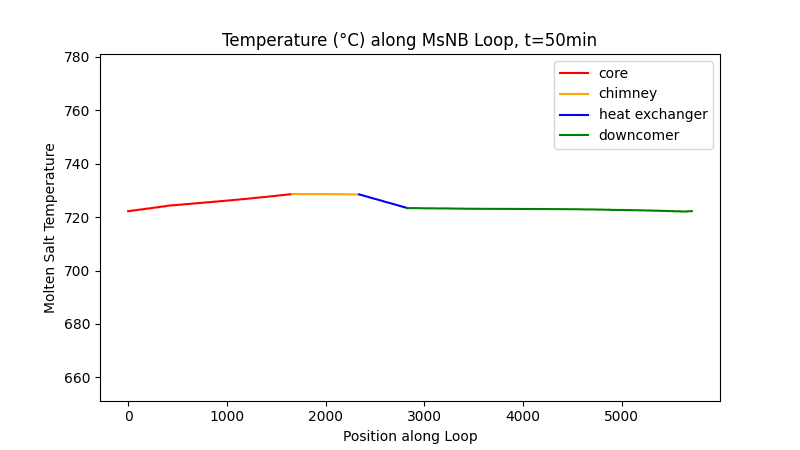
\includegraphics[width=0.49\textwidth]{Simulator/StartUp/Control/animateTx_t/t-50}}
    \quad
    \subfloat[\centering Full-Power]{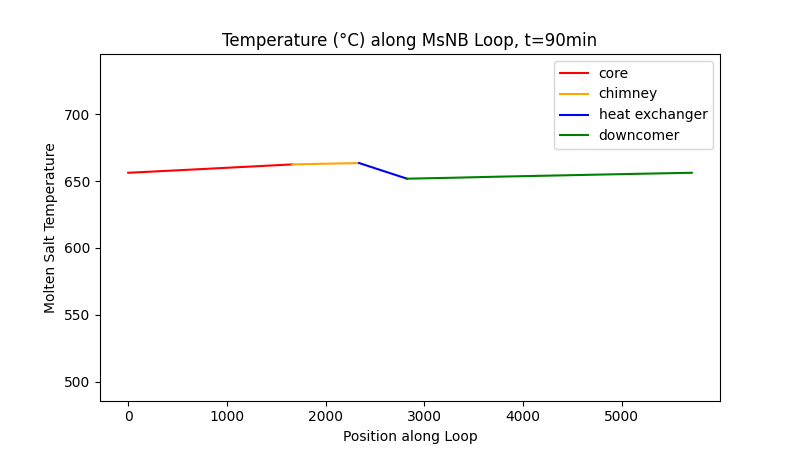
\includegraphics[width=0.49\textwidth]{Simulator/StartUp/Control/animateTx_t/t-90}}
    \subfloat[\centering Steady State]{\includegraphics[width=0.49\textwidth]{Simulator/StartUp/Control/animateTx_t/t-120}}
    \caption[Controlled Start-Up Temperature Profile Response]{Temperature profile response to a controlled start-up from hot-standby.
    \begin{enumerate*}[label=\alph*)]
        \item \acs{msnb} is at hot-standby;
        \item \acs{msnb} has equilibrated at 1 MW;
        \item \acs{msnb} has just reached 10 MW; 
        \item \acs{msnb} has equilibrated at 10 MW;
    \end{enumerate*}}
    \label{fig:Start-Temp-Ctr}
\end{figure}

\subsection{Shut-Down}
The next transient of study is a non-emergency shut-down. The \acs{msnb} is ramped from full-power to low-power, then to hot-standby over the course of 2.5 hours. 

\subsubsection{Autonomous Response}
Figure \ref{fig:Stop-Power-Auto} depicts a rather responsive shut-down, initially. However, as the power decreases, the flow rate slows and flow reactivity resists, and the core power lags behind the heat exchanger. This occurs both during the first ramp and the second ramp. As the core lags the heat exchanger, the salt accumulates sensible heat, which can be observed by the temperature profile rising as is flattens in Figure \ref{fig:Stop-Temp-Auto} and the animation in the supplementary materials\footnotemark[2]. The key metrics for the first ramp are:

\begin{itemize}
    \item Delay Time - 4 min;
    \item Rise Time - 33 min;
    \item Settling Time - 61 min;
    \item Oscillation Period - 22 min;
    \item Inverse Response - 0.0\%;
    \item First Overshoot - 6.2\%;
    \item Second Overshoot -  2.6\%;
\end{itemize}

The second ramp is not as responsive as the first. The temperature profile (see Figure \ref{fig:Stop-Temp-Auto} (b)) has already flattened significantly, so the flow feedback response is very sensitive to subsequent deceleration, and the descent to hot-standby is resisted for the entire duration of the ramp.  The key metrics for the second ramp are:

\begin{itemize}
    \item Delay Time - 14 min;
    \item Rise Time - 33 min;
    \item Settling Time - 45 min;
    \item Oscillation Period - 100 min;
    \item Inverse Response - 22.2\%;
    \item First Overshoot - 8.9\%;
    \item Second Overshoot -  3.3\%;
\end{itemize}

\begin{figure}[ht!]
    \centering
    \includegraphics[width=0.9\textwidth]{Simulator/ShutDown/Auto/t_vs_Qt}
    \caption[Autonomous Shut-Down Power Response]{Core power response for a shut-down from full-power to hot-standby. The heat exchanger power is ramped from 10 MW to 1 MW, then to 100 kW over two separate thirty minute periods.}
    \label{fig:Stop-Power-Auto}
\end{figure}

It would be preferable to counteract the increased flow reactivity with control reactivity instead of temperature reactivity. The flow loop heats up to about 80 \textsuperscript{o}C hotter than the desired core outlet temperature to stabilize the \acs{msnb} as it approaches hot-standby. Allowing this could potentially require requalification of structural materials or even selection of more exotic alloys.

\begin{figure}[!ht]
    \centering
    \subfloat[\centering Full-Power]{\includegraphics[width=0.49\textwidth]{Simulator/ShutDown/Auto/animateTx_t/t-1}}
    \subfloat[\centering Low Power]{\includegraphics[width=0.49\textwidth]{Simulator/ShutDown/Auto/animateTx_t/t-60}}
    \quad
    \subfloat[\centering Heat Exchanger at Hot-Standby]{\includegraphics[width=0.49\textwidth]{Simulator/ShutDown/Auto/animateTx_t/t-120}}
    \subfloat[\centering Core at Hot-Standby]{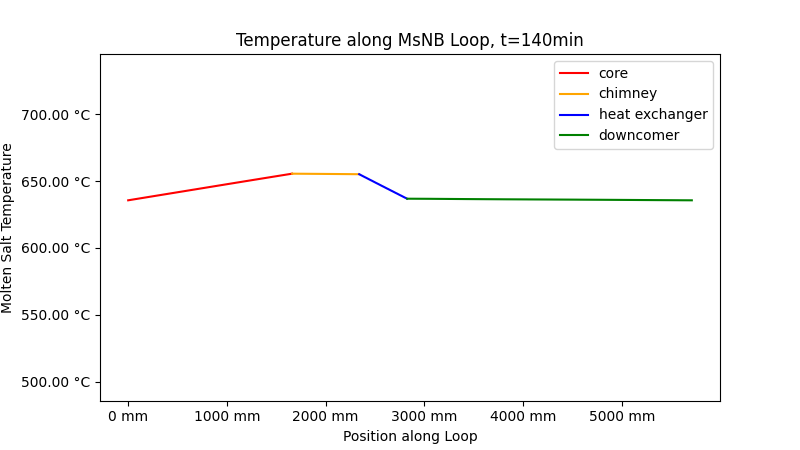
\includegraphics[width=0.49\textwidth]{Simulator/ShutDown/Auto/animateTx_t/t-140}}
    \caption[Autonomous Shut-Down Temperature Profile Response]{Temperature profile response to a shut-down from full-power to hot-standby.
    \begin{enumerate*}[label=\alph*)]
        \item \acs{msnb} is at full-power;
        \item \acs{msnb} has equilibrated at 1 MW;
        \item Heat exchanger has just reached hot-standby; 
        \item Core has equilibrated at hot-standby;
    \end{enumerate*}}
    \label{fig:Stop-Temp-Auto}
\end{figure}


\subsubsection{Controller Response}

\begin{figure}[ht!]
    \centering
    \includegraphics[width=0.9\textwidth]{Simulator/ShutDown/Control/t_vs_Qt}
    \caption[Controlled Shut-Down Power Response]{Core power response for a shut-down from full-power to hot-standby. The heat exchanger power is ramped from 10 MW to 1 MW, then to 100 kW over consecutive 30 minute periods.}
    \label{fig:Stop-Power-Ctr}
\end{figure}

As evidenced by the overlapping orange and blue lines in Figure \ref{fig:Stop-Power-Ctr}, the controller is able to track the set-point nearly perfectly for this shut-down, and is able to eliminate the low-power hold as it brings the \acs{msnb} down to hot-standby. For each ramp, the core power follows the heat exchanger tightly, and settles almost immediately after the heat exchanger transient concludes. The key metrics for the first ramp are:

\begin{itemize}
    \item Delay Time - 4 min;
    \item Rise Time - 28 min;
    \item Settling Time - 30 min;
    \item Oscillation Period - 10 min;
    \item Inverse Response - 0.0\%;
    \item First Overshoot - 2.8\%;
    \item Second Overshoot -  0.0\%;
\end{itemize}

\begin{figure}[!ht]
    \centering
    \subfloat[\centering Full-Power]{\includegraphics[width=0.49\textwidth]{Simulator/ShutDown/Control/animateTx_t/t-1}}
    \subfloat[\centering Low Power]{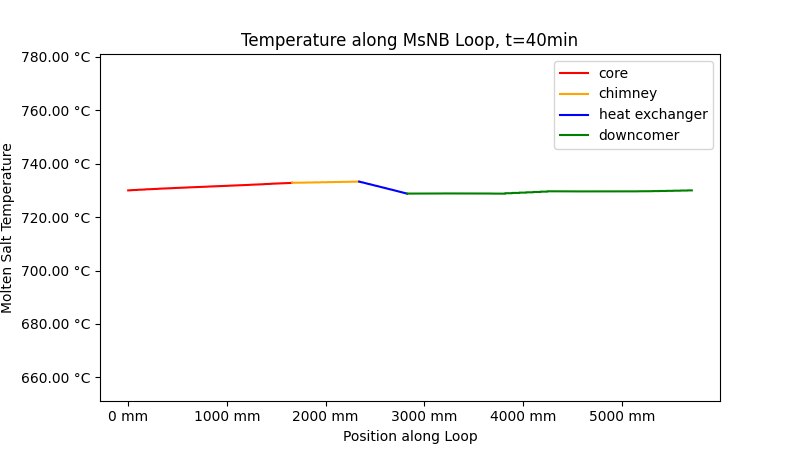
\includegraphics[width=0.49\textwidth]{Simulator/ShutDown/Control/animateTx_t/t-40}}
    \quad
    \subfloat[\centering Heat Exchanger at Hot-Standby]{\includegraphics[width=0.49\textwidth]{Simulator/ShutDown/Control/animateTx_t/t-60}}
    \subfloat[\centering Core at Hot-Standby]{\includegraphics[width=0.49\textwidth]{Simulator/ShutDown/Control/animateTx_t/t-120}}
    \caption[Controlled Shut-Down Temperature Profile Response]{Temperature profile response to a controlled shut-down from full-power to hot-standby.
    \begin{enumerate*}[label=\alph*)]
        \item \acs{msnb} is at full-power;
        \item \acs{msnb} has reached 1 MW;
        \item Heat exchanger has just reached hot-standby; 
        \item Core has equilibrated at hot-standby;
    \end{enumerate*}}
    \label{fig:Stop-Temp-Ctr}
\end{figure}

The key metrics for the first ramp are:

\begin{itemize}
    \item Delay Time - 2 min;
    \item Rise Time - 33 min;
    \item Settling Time - 38 min;
    \item Oscillation Period - 29 min;
    \item Inverse Response - 0.0\%;
    \item First Overshoot - 4.4\%;
    \item Second Overshoot - 3.3\%;
\end{itemize}

Figure \ref{fig:Stop-Temp-Ctr} and the animation in the supplementary materials show that the more responsive shut-down caused by the controller led to more favorable temperature profile dynamics. The hot-standby temperature was implicitly controlled to exceed the full-power core outlet temperature by just 9 \textsuperscript{o}C, which is well within normal operating range, and represents a significant improvement over the autonomous response.


\subsection{Demand-Response}
The final transient of study is a demand-response that may be required of an \acs{msnb} that is coupled to a solar farm. On a cloudy day,photovoltaic solar panels reduce their effectiveness to between 20\% and 70\% depending on how cloudy the sky is. If a single cloud passes over the sun, it is assumed that the effectiveness drops to the high end of that spectrum, and a 2 MW solar power plant may reduce its output by about 600 kW. Assuming a power conversion efficiency of about 30\%, the \acs{msnb} may then be asked to ramp up by 2 MW for a short period so that the entire system can meet demand.  It is assumed that it takes 5 minutes for the cloud to fully cover the sun, it passes over in 10 minutes, and it takes another 5 minutes to uncover the sun.

\subsubsection{Autonomous Response} 

\begin{figure}[ht!]
    \centering
    \includegraphics[width=0.9\textwidth]{Simulator/DemandResponse/Auto/t_vs_Qt}
    \caption[Autonomous Demand-Response Power Response]{Core power response to a heat exchanger demand transient. The \acs{msnb} is ramped from 8 MW to 10 MW over 5 minutes, holds for 10 minutes, then is ramped back to 8 MW in 10 minutes.}
    \label{fig:Demand-Power-Auto}
\end{figure}

The passive feedback mechanisms alone are not sufficient to follow such a load profile. Though the transient does not destabilize the reactor, Figure \ref{fig:Demand-Power-Auto} displays large overshoots that do not lend themselves to power peaking. The \acs{msnb} never settles at the temporarily required full-power. The key metrics for the first ramp are:

\begin{itemize}
    \item Delay Time - 3 min;
    \item Rise Time - 5 min;
    \item Settling Time - N/A min;
    \item Oscillation Period - 7 min;
    \item Inverse Response -2.5\%;
    \item First Overshoot - 41.0\%;
    \item Second Overshoot - 23.0\%;
\end{itemize}

\begin{figure}[ht!]
    \centering
    \includegraphics[width=0.9\textwidth]{Simulator/DemandResponse/Auto/auto_reac_phase}
    \caption[Autonomous Demand-Response Reactivity Phase Space]{Passive reactivity phase space response to a heat exchanger demand heat exchanger demand transient. The \acs{msnb} is ramped from 8 MW to 10 MW over 5 minutes, holds for 10 minutes, then is ramped back to 8 MW in 10 minutes.}
    \label{fig:Demand-PassivePhase-Auto}
\end{figure}

The key metrics for the second ramp are shaped by fact that the core power happens to be dropping when the sun begins exiting the cloud. If it were rising, the response to the ramp-down, particularly until the first overshoot, may look very different:

\begin{itemize}
    \item Delay Time - 0.5 min;
    \item Rise Time - 5.2 min;
    \item Settling Time - 33 min;
    \item Oscillation Period - 8 min;
    \item Inverse Response - 0.0\%;
    \item First Overshoot - 32.0\%;
    \item Second Overshoot - 18.5\%;
\end{itemize}

Figure \ref{fig:Demand-PassivePhase-Auto} is a passive feedback phase space representation of the transient. The \acs{msnb} hovers around unity until the heat exchanger begins delivering more power to the secondary working fluid. Flow reactivity then makes the core subcritical, causing the inverse response, before the cold salt reaches the core and it ramps up. When the heat exchanger ramp stops, the reactor twice circulates a different point along the diagonal in a large loop primarily driven by thermal density wave oscillations traversing the flow loop. When the heat rejected begins ramping back down, the passive reactivity phase space curve happens to be below the diagonal, otherwise it would take some additional time for the deceleration of the salt to ramp the reactor back down to low power. Once the heat exchanger settles back to 80\% of full power, the core spirals around the original unity point as it settles back to the original power level.

\subsubsection{Controller Response}
\begin{figure}[ht!]
    \centering
    \includegraphics[width=0.9\textwidth]{Simulator/DemandResponse/Control/t_vs_Qt}
    \caption[Controlled Demand-Response Power Response ]{Controlled core power response to a heat exchanger demand transient. The \acs{msnb} is ramped from 8 MW to 10 MW over 5 minutes, holds for 10 minutes, then is ramped back to 8 MW in 10 minutes.}
    \label{fig:Demand-Power-Ctr}
\end{figure}

\begin{figure}[ht!]
    \centering
    \includegraphics[width=0.9\textwidth]{Simulator/DemandResponse/Control/contr_reac_phase}
    \caption[Controlled Demand-Response Reactivity Phase Space]{Controlled reactivity phase space response to a heat exchanger demand heat exchanger demand transient. The \acs{msnb} is ramped from 8 MW to 10 MW over 5 minutes, holds for 10 minutes, then is ramped back to 8 MW in 10 minutes.}
    \label{fig:Demand-ControlPhase-Ctr}
\end{figure}
\clearpage